\section{Methodology} \label{sec:method}

To address the identified gaps and support the goal of designing efficient, reliable, and safe LT-PEMFC systems for aircraft, the authors are developing:

\begin{enumerate}
	\item Dynamic multi-scale and multi-physics LT-PEM cell models.
	\item Parametric stack, TMS, WMS, fuel supply, and air supply models.
	\item Advanced physics-aware machine learning LT-PEMFC stack surrogates.
	\item A computational framework for dynamic fuel cell system modelling.
	\item Advanced computational methods to efficiently explore optimal system design.
\end{enumerate}

Together these actions aim to help the community understand the impact of LT-PEMFC power system transients at take-off, and begin tackling challenges surrounding the integration of these systems on board future large transport aircraft.

\subsection{Cell Modelling}

The physical processes necessary for the operation of LT-PEMFCs occur across a wide range of length scales. The catalysed ORR at a three-phase boundary and transport of water across the ionomer are governed by molecular level physics. Simultaneously the convective transport of reactants occurs first over the cell width, and second, through pores of diameter smaller than the mean free path of the gas molecules. These multi-scale mass, momentum, species, charge, and energy transfers are tightly coupled, resolving them fully is infeasible with current computational capability.

\noindent
\begin{minipage}[t]{\linewidth}
	\begin{align}
		\frac{\partial(\epsilon C_k)}{\partial t} + \nabla (\vec{u} + C_k)                                        & = \nabla(D_k^{\text{eff}} \nabla C_k) + S_k               & \frac{\partial(\rho c_p)_mT}{\partial t} + \nabla(\rho c_p \vec{u} T) & = \nabla(k_{\text{eff}} \nabla T) + S_T \tag{3a, 3b} \\
		\frac{1}{\frac{\partial( \epsilon \rho \vec{u})}{\partial t}  + \frac{1}{\nabla (\rho \vec{u} \vec{u})} } & = -\nabla p + \nabla \tau + S_u                           &
		\frac{\partial(\epsilon \rho)}{\partial t} + \nabla(\rho \vec{u})                                         & = S_m                                        \tag{4a, 4b}                                                                                                                                \\
		\nabla(\kappa^{\text{eff}} \nabla \Phi_e)                                                                 & = -S_\Phi                                                 &
		\nabla(\sigma^{\text{eff}}\nabla\Phi_s)                                                                   & = S_\Phi \tag{5a, 5b}
	\end{align}
\end{minipage}%
\hfill\vspace{1em}
\begin{minipage}[t]{\linewidth}
	\begin{center}
		\captionof{table}{Source terms for the single-phase fuel cell model presented by [wang]}
		\newcolumntype{V}{>{\hsize=.4\hsize}>{\raggedright\arraybackslash}X}
		\newcolumntype{Y}{>{\centering\arraybackslash}X}
		\newcolumntype{Z}{>{\hsize=.5\hsize}>{\centering\arraybackslash}X}
		\begin{tabularx}{\linewidth}{V Z Y Z}
			\toprule
			                & Gas Diffusion Layer             & Catalyst Layer                                                                      & Membrane                                  \\
			\midrule
			Mass (4b)       &                                 & $S_m = \sum_k M_k S_k + M_{\water} \nabla (D_{w,m} \nabla C_{\water})$              &                                           \\
			Momentum (4a)   & $S_u = -\vec{u}(\frac{\mu}{K})$ & $S_u = -\vec{u}(\frac{\mu}{K})$                                                     & $\vec{u} = 0$                             \\
			Species (3a)    &                                 & $S_k = -\nabla\left( \frac{n_d}{F} i_e\right) - \left( \frac{s_k j}{nF}\right)$     & $-\nabla\left( \frac{n_d}{F} i_e\right)$  \\
			Charge (5a, 5b) &                                 & $S_\Phi = j$                                                                        &                                           \\
			Energy (3b)     &                                 & $S_T = j\left( \eta + T \frac{dU_0}{dT}\right) + \frac{i_e^2}{\kappa^{\text{eff}}}$ & $S_T = \frac{i_e^2}{\kappa^{\text{eff}}}$ \\
			\bottomrule
		\end{tabularx}
	\end{center}
\end{minipage}

Commonly, when investigating cell and stack polarisation, assumptions of continuity allow diffusive processes to be modelled without resolving pore scale effects. This allows for the derivation of Partial Differential Equations (PDEs) commonly solved via finite element methods and finite volume methods. Often, a single set of equations is applied over the full domain of a cell, with the response of different subdomains governed by their source terms. One such set of PDEs, presented by [wang], is given in table 2. A wide range of PDEs of differing fidelities are presented throughout literature, trading computational cost against physics complexity.

Open-source fuel cell models are of interest in this work as they provide an efficient approach to incorporating multiple model fidelities. A non-exhaustive list of open-source models are presented in table [].

\begin{center}
	\begin{table}
		\caption{Do This}
		\newcolumntype{Y}{>{\centering\arraybackslash}X}
		\newcolumntype{Z}{>{\hsize=.65\hsize}>{\centering\arraybackslash}X}
		\newcolumntype{V}{>{\hsize=.4\hsize}>{\centering\arraybackslash}X}
		\begin{tabularx}{\linewidth}{V Y Z Z Z Z}
			\toprule
			Authors     & Vetter \& Schumacher & Secanell \etal & Zhang \etal & Kone \etal & Gass \etal \\
			\midrule
			Dimension   & One                  & Up to three    & Three       & Three      & One        \\
			Isothermal  &                                                                               \\
			Water Phase & Multi                & Multi          & Multi       & Single     & Multi      \\
			\bottomrule
		\end{tabularx}
		\label{tab:opensource}
	\end{table}
\end{center}

\subsection{Surrogate Modelling}

[Autoregressive Multi-fidelity GPs]

[Active learning, and Bayesian Optimisation]

[Non-myopic Bayesian optimisation]

[Proposed Fuel Cell Stack Surrogate]

\subsection{Dynamic Fuel Cell System Model}

A computational framework for dynamic fuel cell system modelling has been developed by the authors to allow modular development and simple composition of fuel cell system component models. This has been accompanied by implementation of the following sub-models from the work of Pukrushpan et al \cite{pukrushpan_control_2004}.
\begin{multicols}{2}
	\begin{itemize}
		\item Electric Motor
		\item Compressor
		\item Manifold
		\item Humidifer
		\item Cathode
		\item Anode
		\item Membrane Hydration
		\item Stack Voltage
	\end{itemize}
\end{multicols}
\vspace{-1em}
The resulting LT-PEMFC power system model has been validated against the work of Pukrushpan et al, as demonstrated in Figures \ref{} and \ref{}.

\noindent
\begin{minipage}[t]{\linewidth}
	\begin{center}
		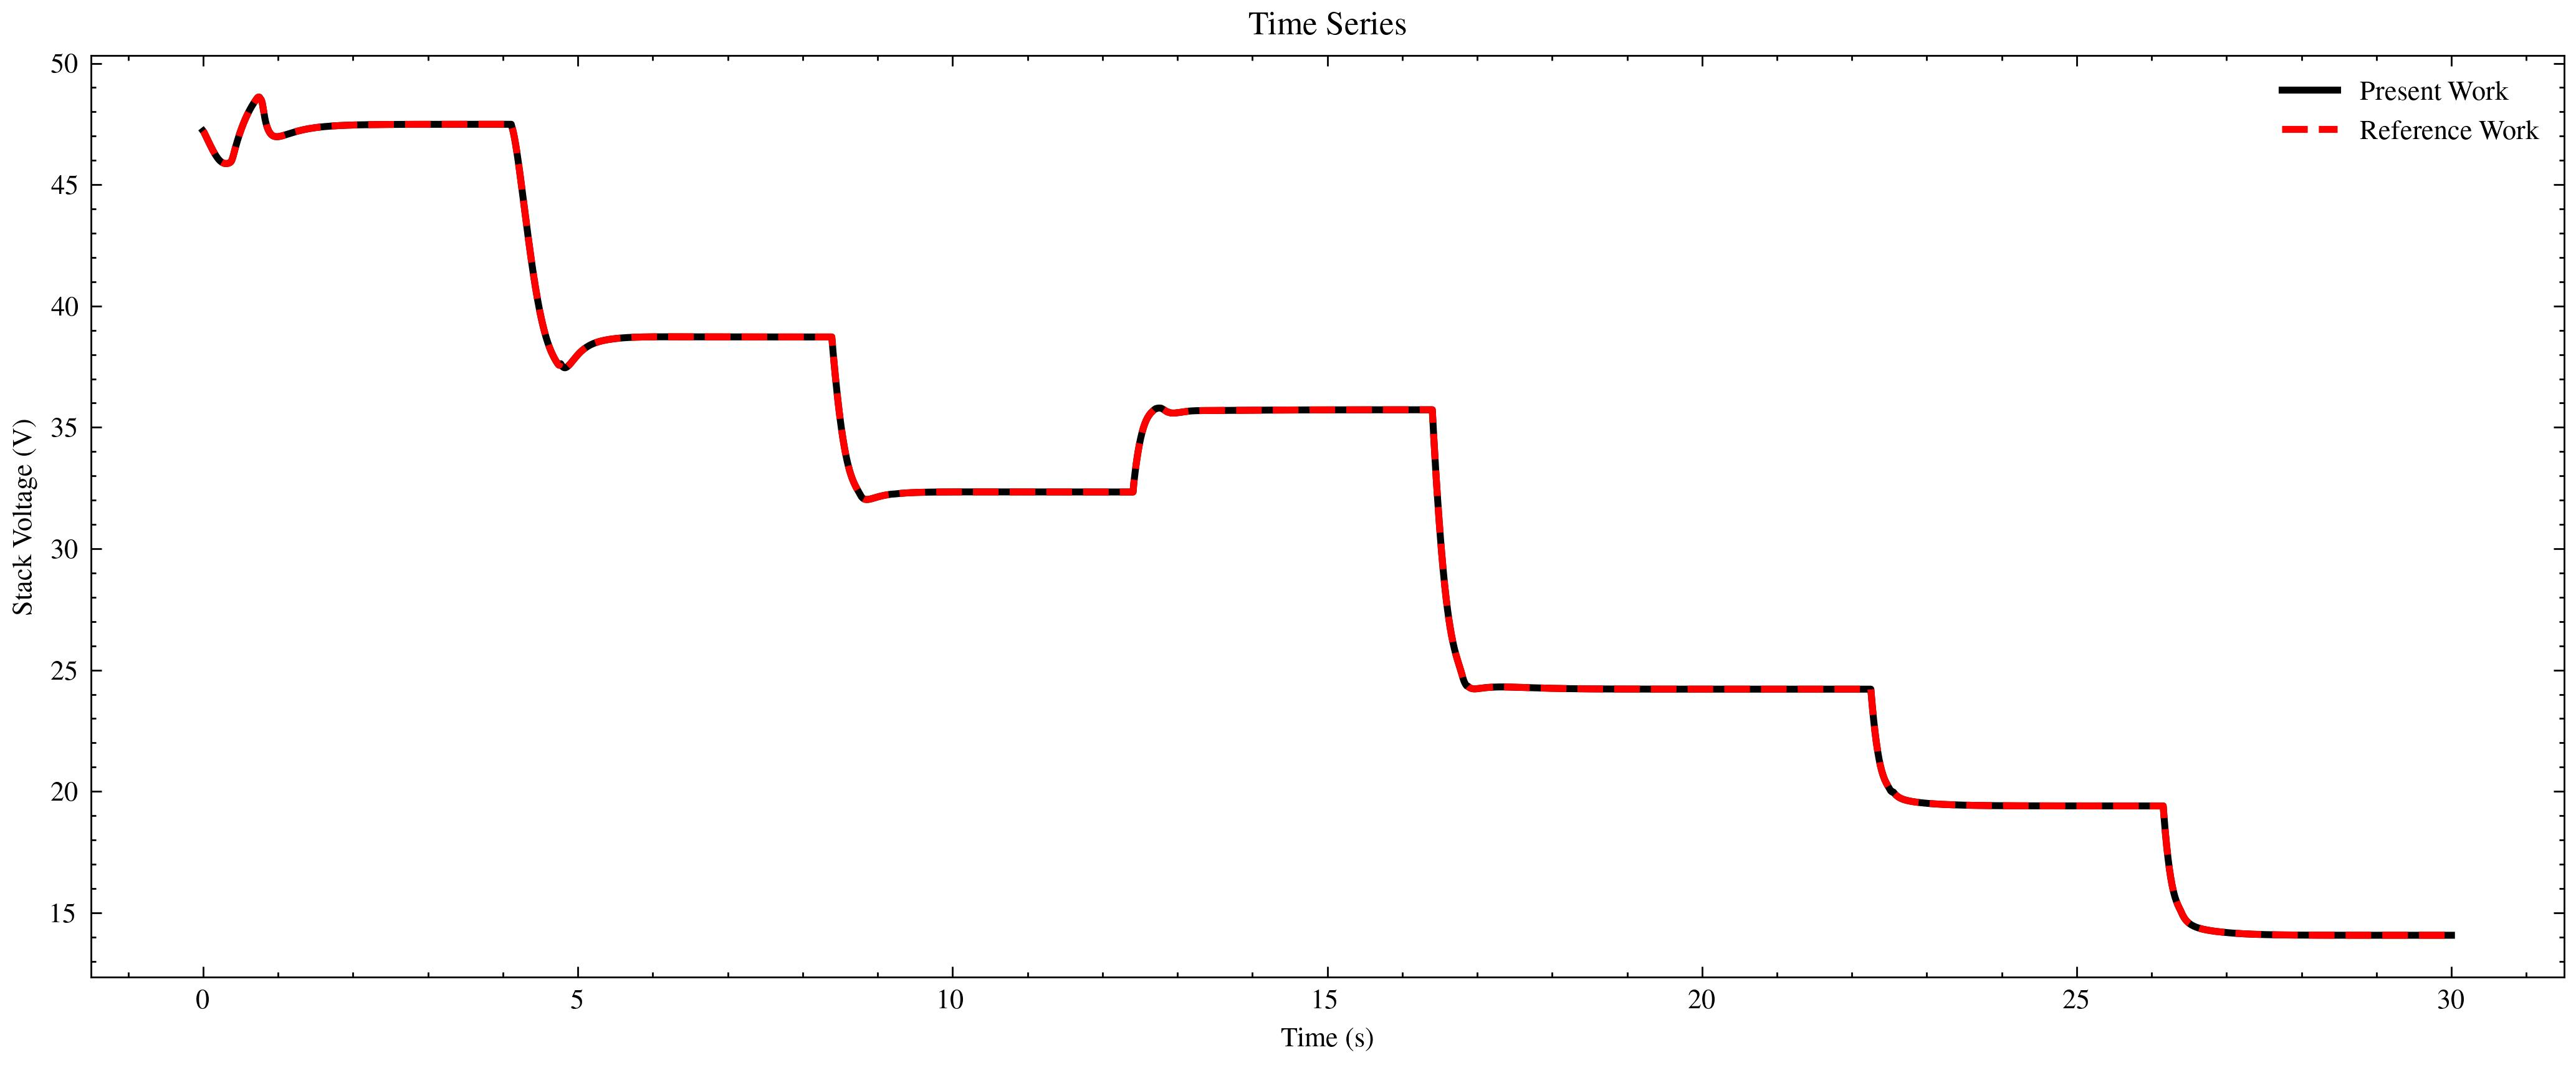
\includegraphics[height=18em]{figures/voltage_ts.jpg}
		\captionof{figure}{Some caption}
	\end{center}
\end{minipage}%
\hfill\vspace{1em}
\begin{minipage}[t]{\linewidth}
	\begin{center}
		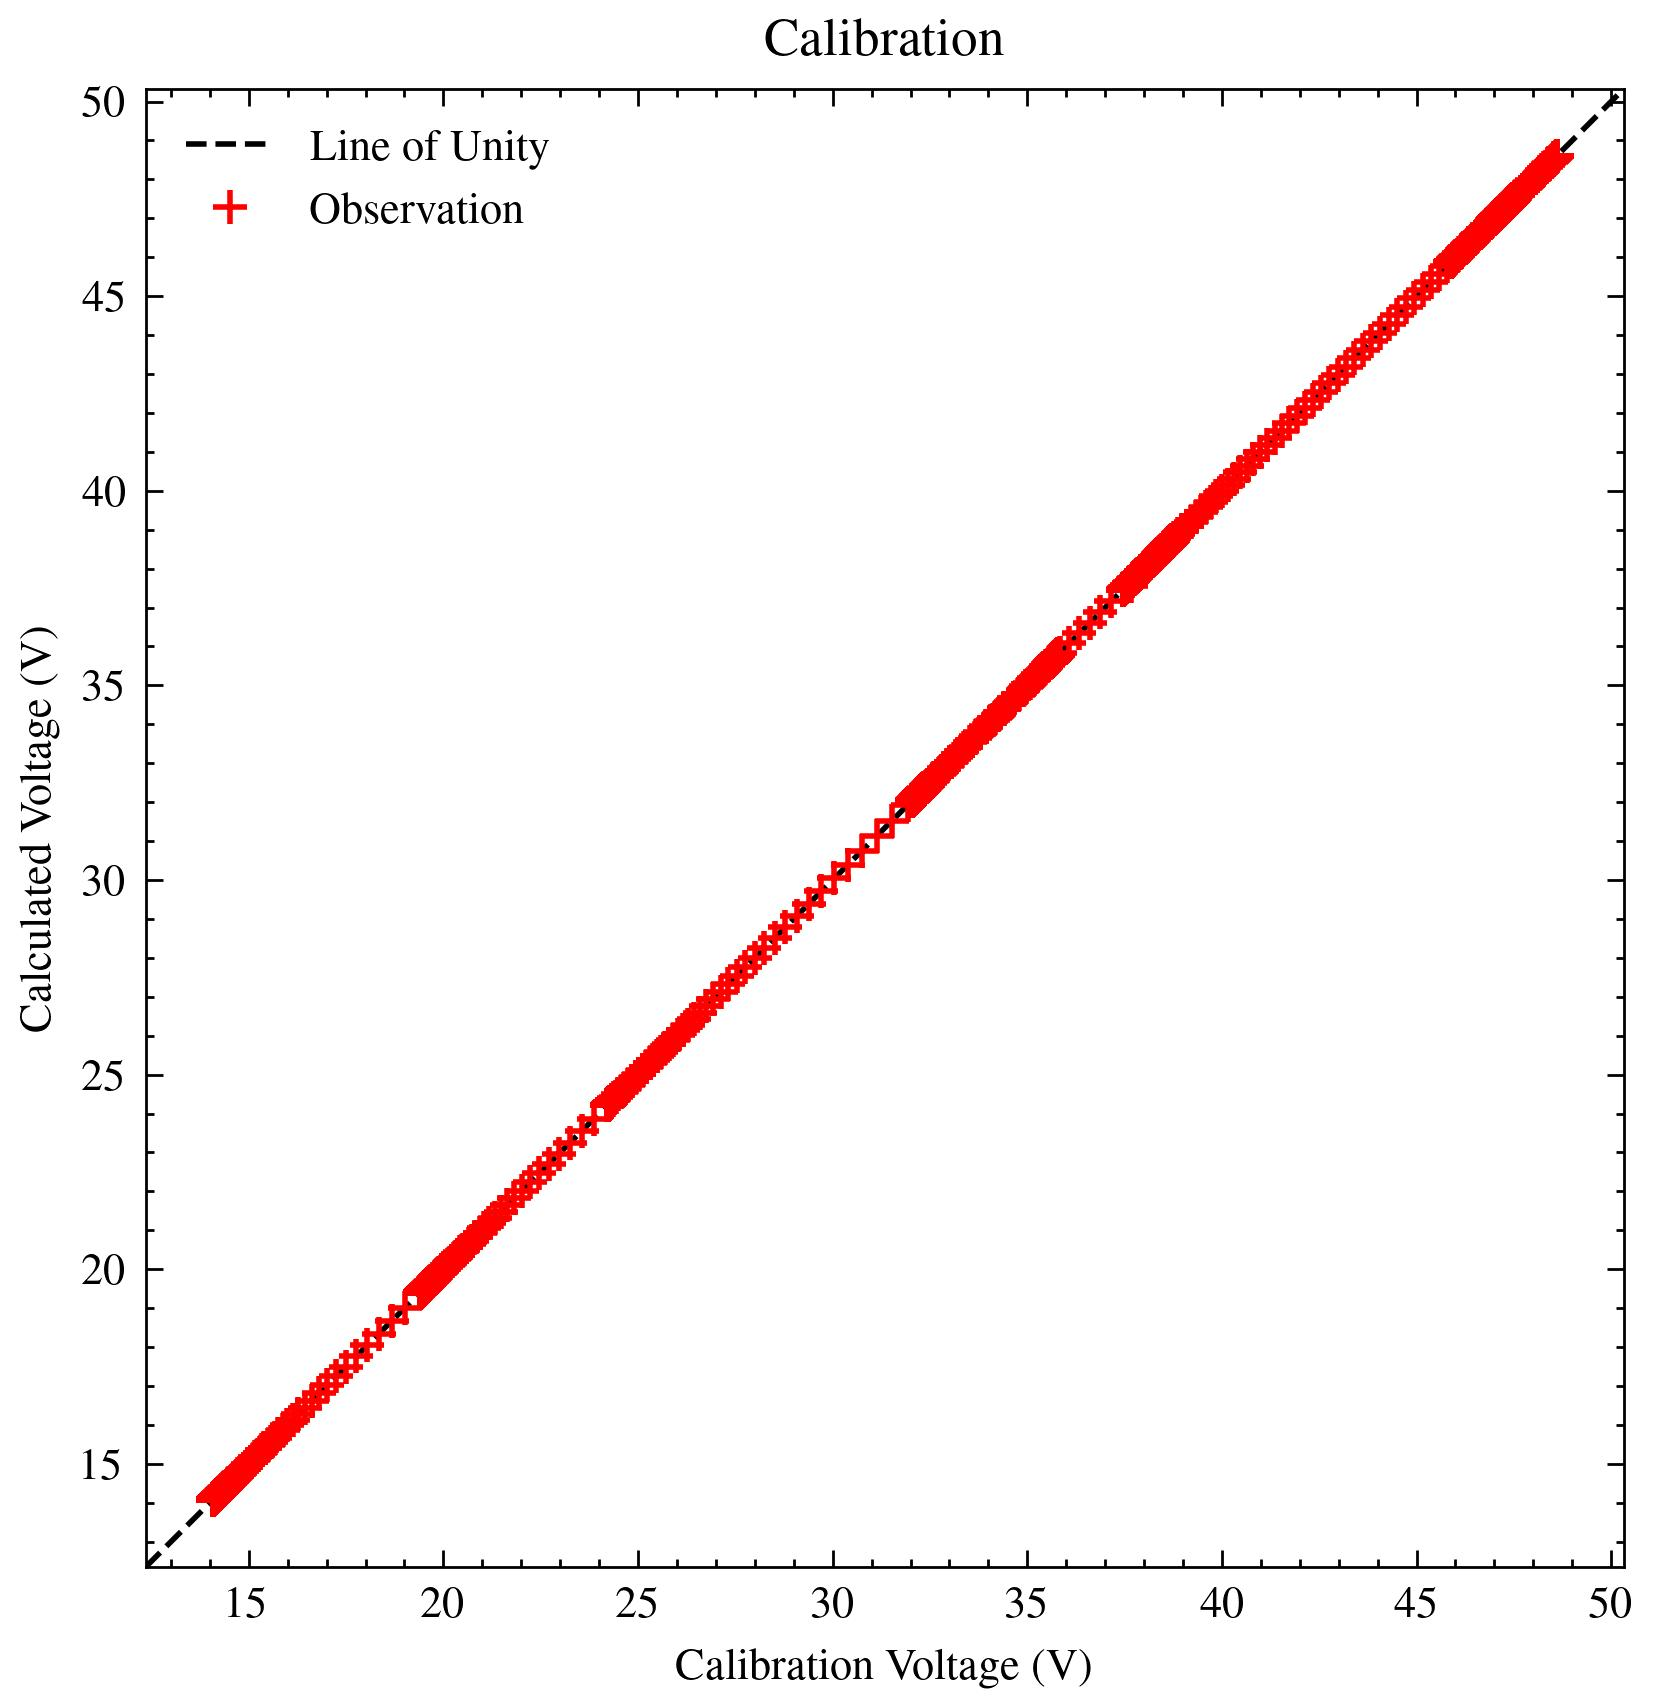
\includegraphics[height=18em]{figures/voltage_cal.jpg}
		\captionof{figure}{Some caption}
	\end{center}
\end{minipage}

Future work is planned to implement sub-models for future LT-PEMFC aircraft systems. This will include water management, thermal management, air supply, and fuel supply systems. The response of a given stack design evaluated using the stack surrogate model described in section []. The system dynamic response is evaluated using an implicit adaptive Runge-Kutta integrator. An XDSM diagram of the proposed study is presented in figure \ref{fig:xdsm}.

\begin{center}
	\begin{figure}
		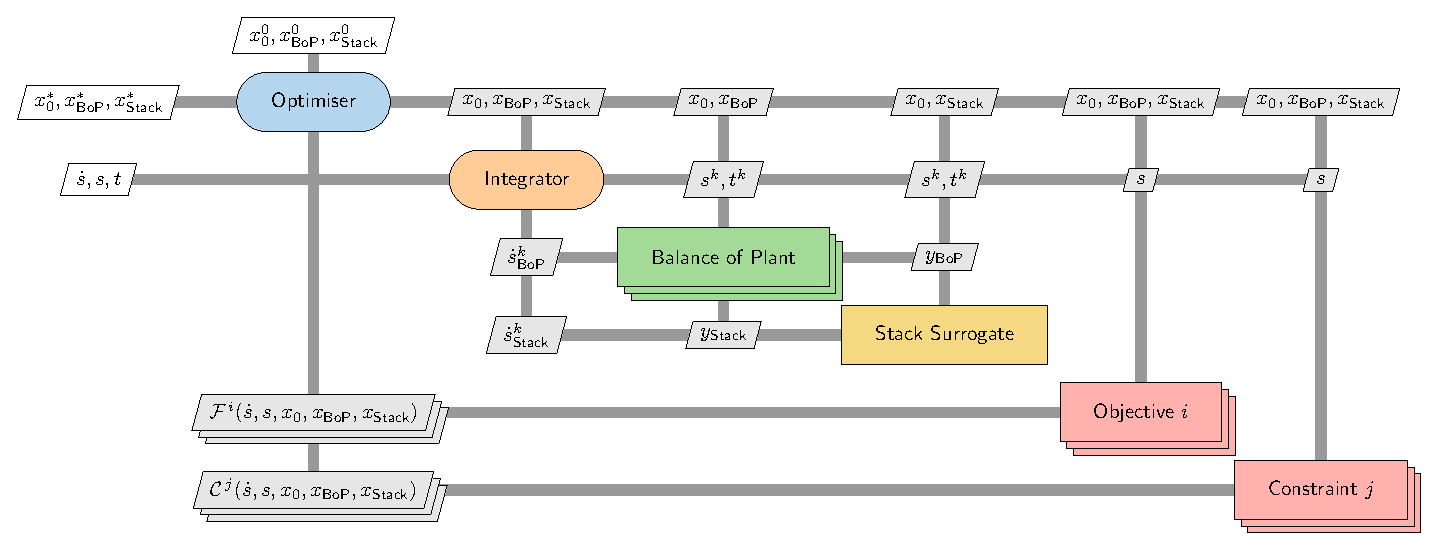
\includegraphics[width=\linewidth]{figures/xdsm.pdf}
		\caption{XDSM Diagram of the proposed fuel cell system model}
		\label{fig:xdsm}
	\end{figure}
\end{center}

\subsection{Design Optimisation}

